\documentclass{article}
\usepackage{amsmath}
\usepackage{amsthm}
\usepackage{amsfonts}
\usepackage{amssymb}
\usepackage{bbold}
\usepackage{dsfont}
\usepackage{graphicx}
\usepackage{cleveref}
\usepackage{bm}
\usepackage{booktabs}
\usepackage{siunitx}
\usepackage{xcolor}
\usepackage{pdfpages}
\usepackage[utf8]{inputenc}
\usepackage[english]{babel}
\newtheorem{definition}{Definition}
\newtheorem{example}{Example}
\newcommand{\exP}[1]{\mathrm{e}^{#1}}
\newcommand{\dif}{\mathrm{d}}
\renewcommand{\vec}[1]{\mathbf{#1}}
\newcommand{\pdagger}{{\phantom{\dagger}}}
\newcommand{\state}[1]{\vert #1\rangle}
\newcommand{\cstate}[1]{\langle #1\vert}
\newcommand{\tr}[1]{\mathrm{tr}\left\{#1\right\}}
\newcommand{\trs}[2]{\, \mathrm{tr}_{#1}\{#2\}}
\newcommand{\expc}[3]{\langle #1\vert #2 \vert #3\rangle}
\usepackage[doi=false,url=false,isbn=false,backend=bibtex,style=nature,natbib=true,sorting=none]{biblatex}
\bibliography{bib.bib}
\usepackage{geometry}
\geometry{
	a4paper,
	total={170mm,257mm},
	left=15mm,
	right=15mm,
	top=15mm,
}
\begin{document}
\title{Report 27: TTHEOM results, variation of electron-vibrational coupling (smaller values)}
\maketitle
\section{Parameters}
\begin{itemize}
	\item $N=1\times 3$
	\item $\varepsilon_0 = -\SI{240}{\milli\electronvolt}$
	\item $\omega_0 = \SI{100}{\milli\electronvolt}$
	\item $t_0=\SI{40}{\milli\electronvolt}$
	\item $\lambda_0=\SI{1}{\milli\electronvolt}$
	\item $\lambda_1=\SI{0.1}{\milli\electronvolt}$
	\item $\Gamma_0=\SI{10}{\milli\electronvolt}$
	\item $k_B T=\SI{25}{\milli\electronvolt}$
	\item $t_1\in[0.2,0.5,0.8]t_0$
	\item $V\in[0.25,0.5,0.75]\SI{}{\volt}$
\end{itemize}
\section{Overview of results}
\begin{itemize}
	\item Comparison of charge current dynamics, spin selectivity, and maximal rank for varying spin-independent electron-vibrational coupling $t_1\in[8,20,32]\si{\milli\electronvolt}$, for three voltage points $V\in[0.25,0.5,0.75]\si{\volt}$ (close to upper electronic band edge, aligned with electronic band center, and close to lower electronic band edge)
	\item Charge current at larger voltage seems to be suppressed for larger electron-vibrational coupling
	\item Spin selectivity is still very small, except for the voltage $V=\SI{0.25}{\volt}$, where there is essentially no transport and the currents are nearly vanishing.  
	\item For a fixed voltage, the maximal rank in the stationary state increases proportional to the dominant electron-vibrational coupling strength.
\end{itemize}
\begin{figure}[!h]
	\centering
	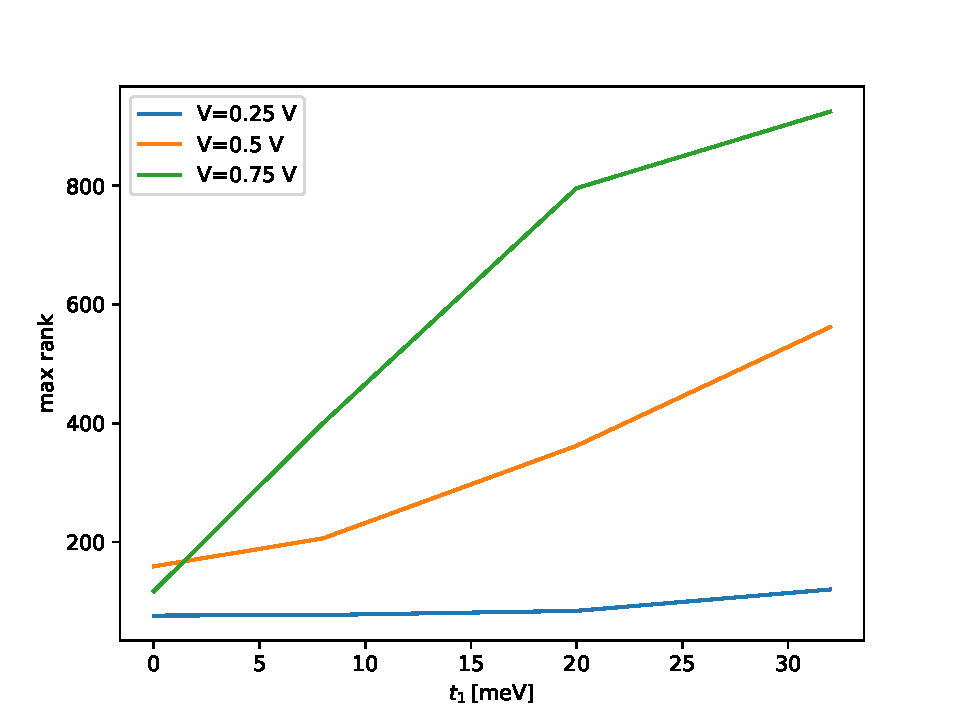
\includegraphics[width=0.7\textwidth]{figs/L1x3_VVar_maxRank_final_nvib5_tol1e-3.pdf}
	\caption{Maximum rank at final time for $n_\mathrm{vib}=5$ and $\mathrm{tol}=10^{-3}$, varying electron-vibrational coupling $t_1$ and voltage $V$.}
\end{figure}
\vspace{10cm}
\section{$t_1=\lambda_1=\SI{0}{\electronvolt}$}
\begin{figure}[!h]
	\centering
	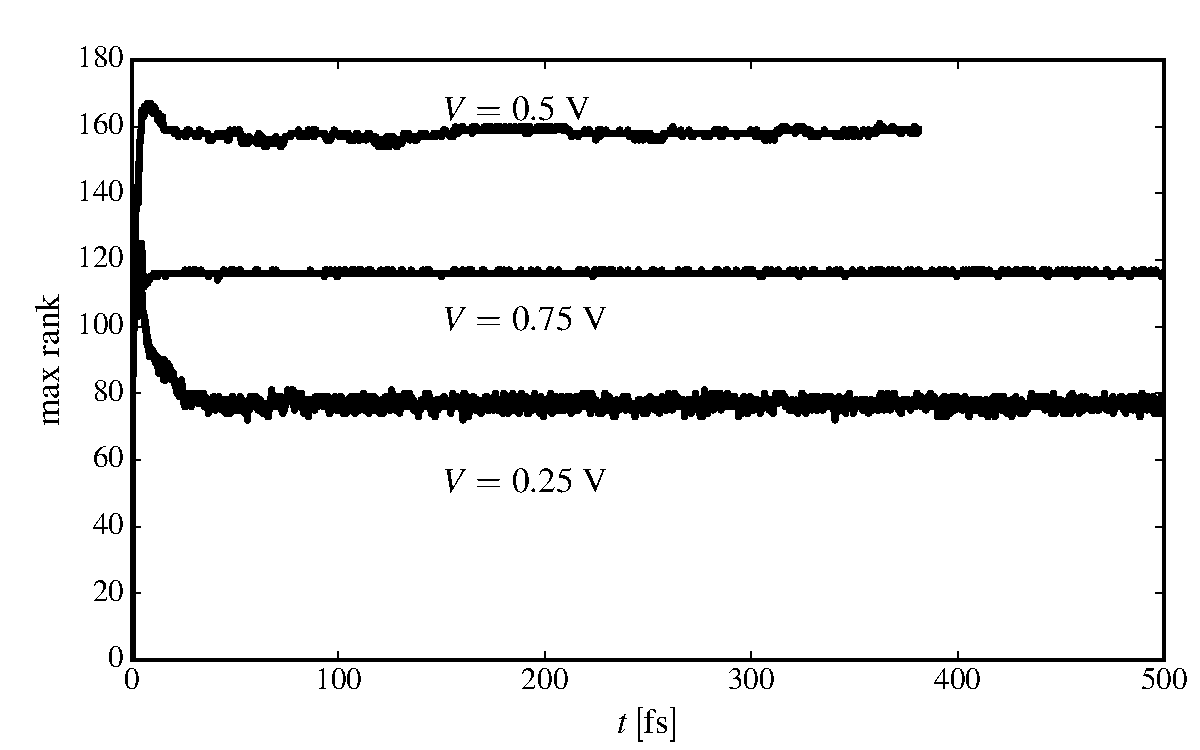
\includegraphics[width=0.7\textwidth]{figs/t1_0/L1x3_t1_0_tamen_maxRank_P_Vvar_nVar_tol1e-3.pdf}
	\caption{Dynamics of the maximal rank for the case that the electron-vibrational coupling is vanishing.}
\end{figure}
\clearpage
\section{$t_1=\SI{8}{\milli\electronvolt}$}
\begin{figure}[!h]
	\centering
	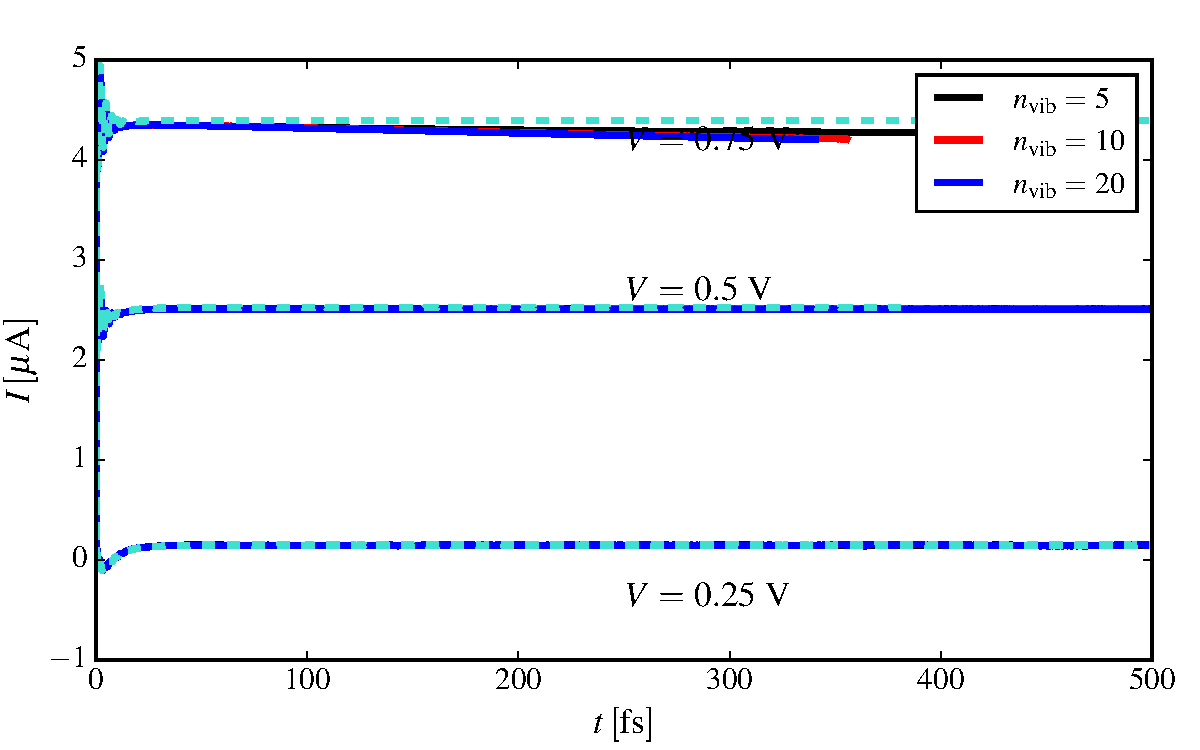
\includegraphics[width=0.54\textwidth]{figs/t1_2/L1x3_t1_2_tamen_cur_P_Vvar_nVar_tol1e-3.pdf}
	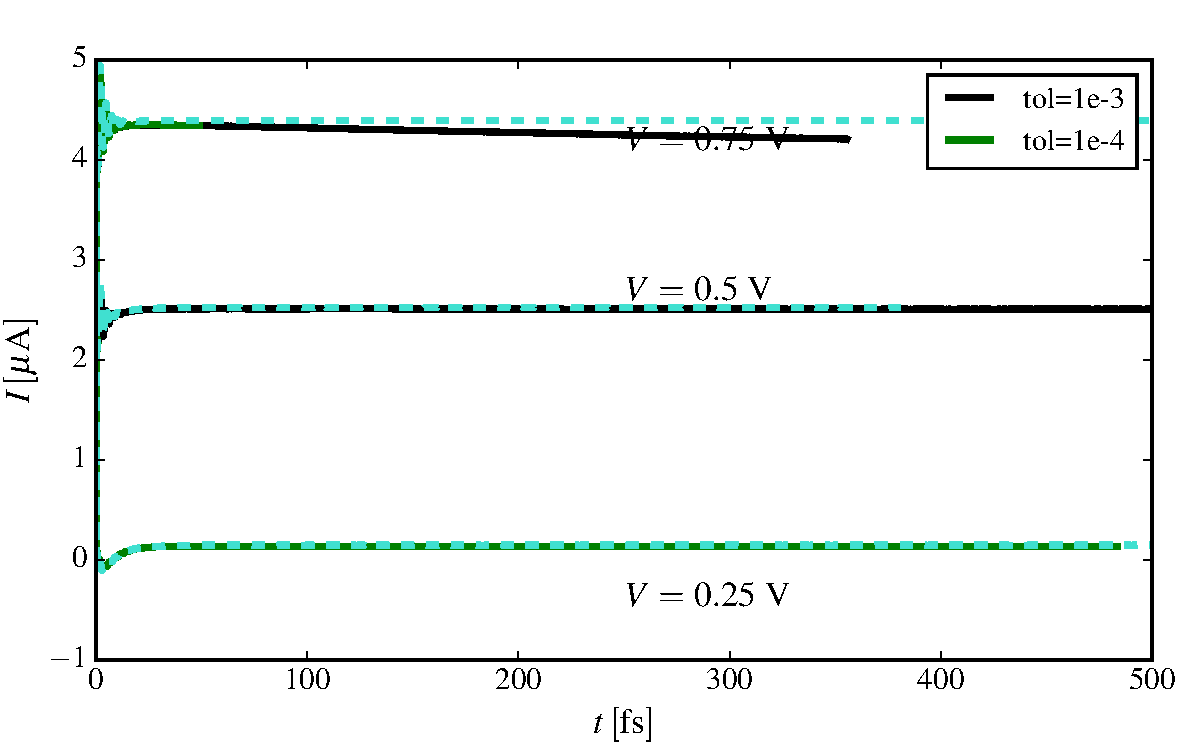
\includegraphics[width=0.54\textwidth]{figs/t1_2/L1x3_t1_2_tamen_cur_P_Vvar_nvib10_tolVar.pdf}
	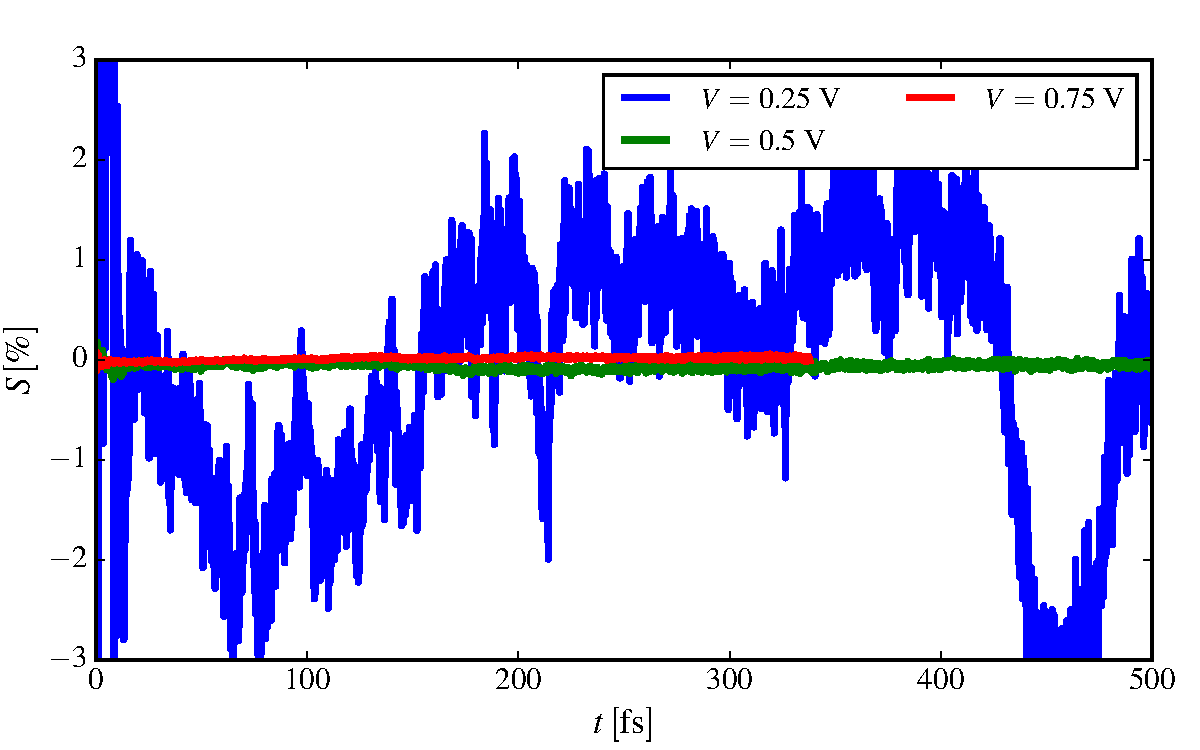
\includegraphics[width=0.54\textwidth]{figs/t1_2/L1x3_t1_2_tamen_SP_Vvar_nv20_tol1e-3.pdf}
	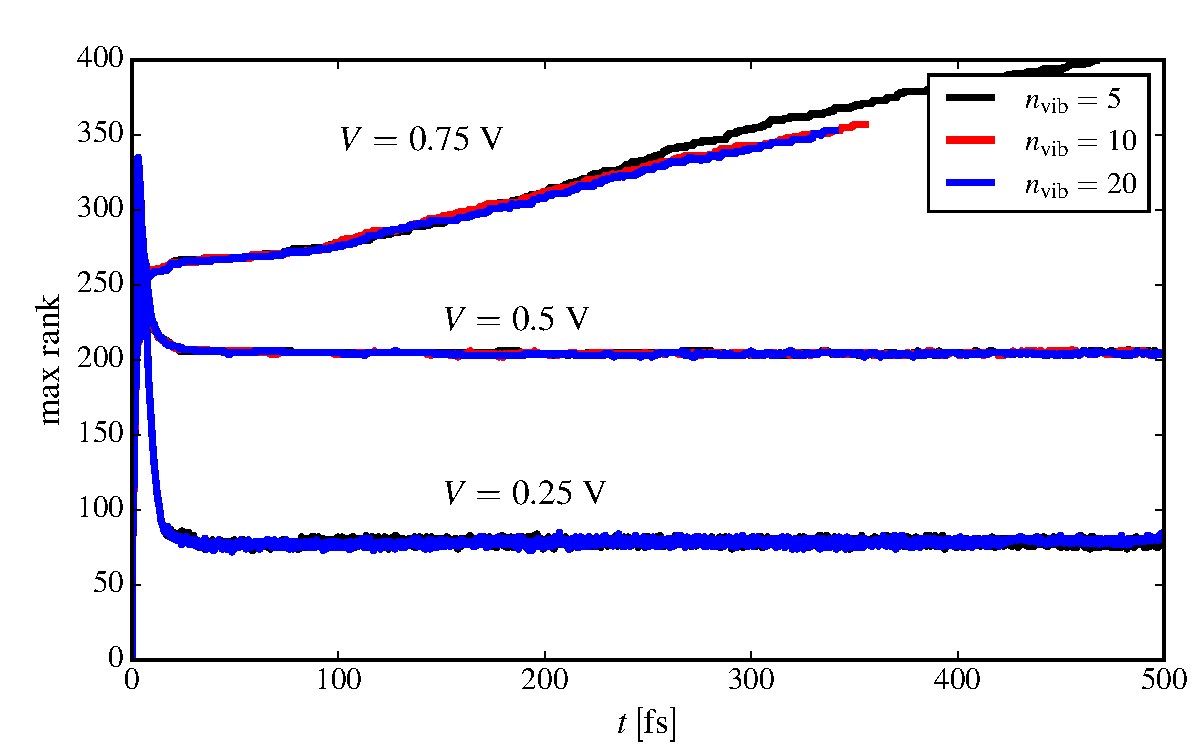
\includegraphics[width=0.54\textwidth]{figs/t1_2/L1x3_t1_2_tamen_maxRank_P_Vvar_nVar_tol1e-3.pdf}
\end{figure}
\clearpage
\section{$t_1=\SI{20}{\milli\electronvolt}$}
\begin{figure}[!h]
	\centering
	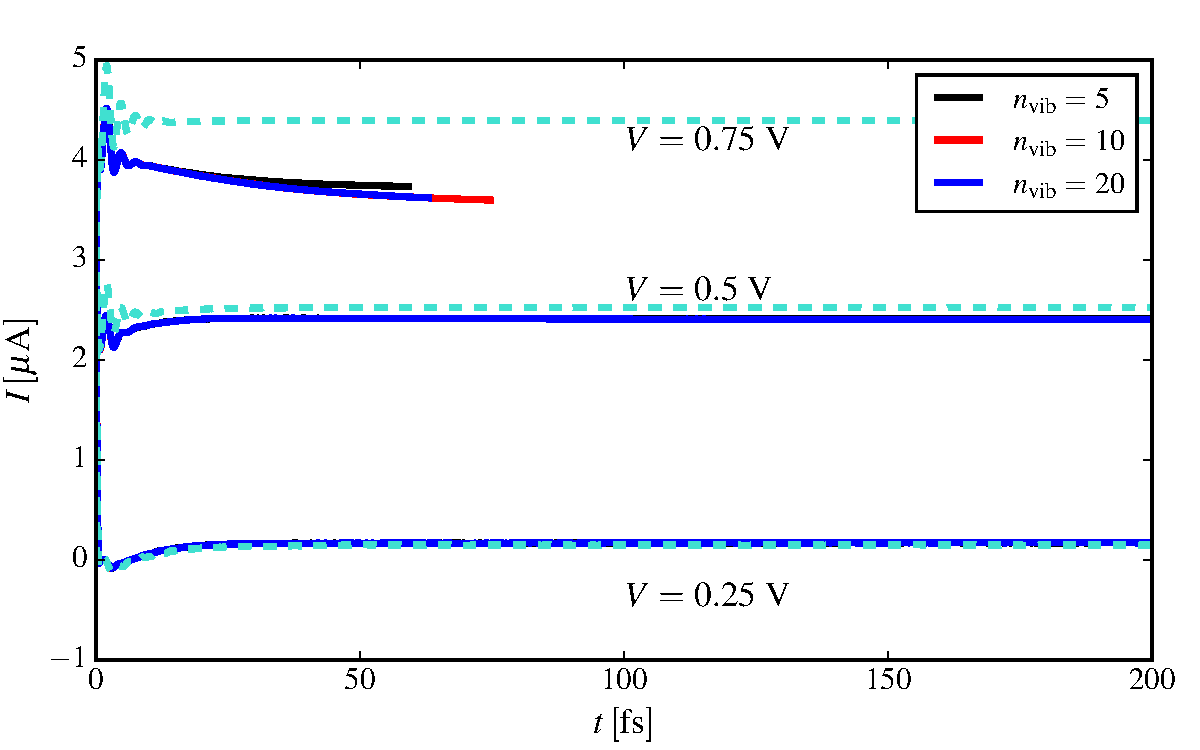
\includegraphics[width=0.54\textwidth]{figs/t1_5/L1x3_t1_5_tamen_cur_P_Vvar_nVar_tol1e-3.pdf}
	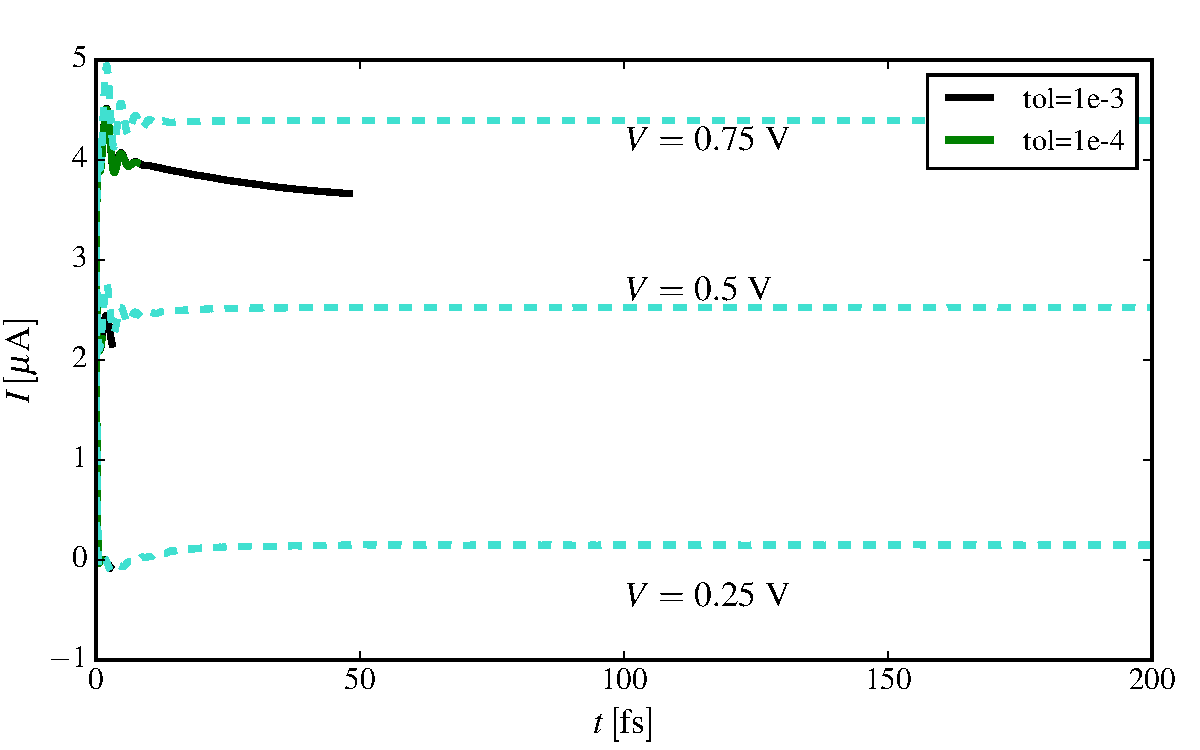
\includegraphics[width=0.54\textwidth]{figs/t1_5/L1x3_t1_5_tamen_cur_P_Vvar_nvib10_tolVar.pdf}
	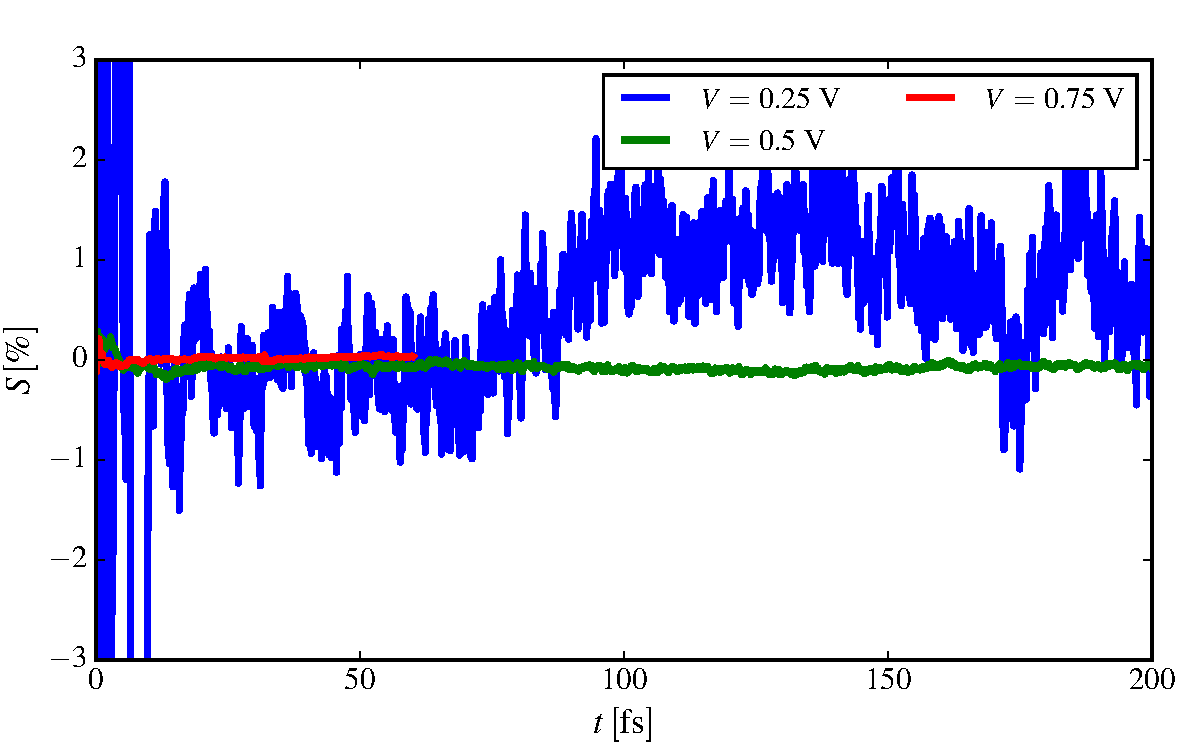
\includegraphics[width=0.54\textwidth]{figs/t1_5/L1x3_t1_5_tamen_SP_Vvar_nv20_tol1e-3.pdf}
	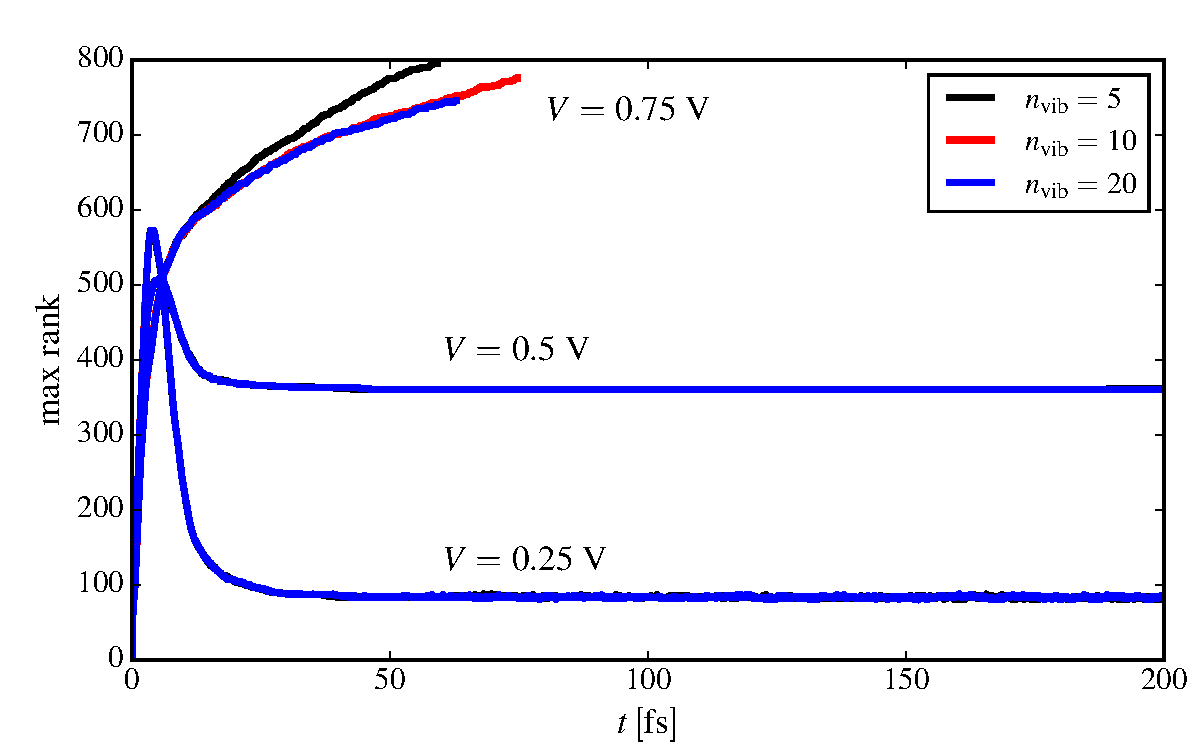
\includegraphics[width=0.54\textwidth]{figs/t1_5/L1x3_t1_5_tamen_maxRank_P_Vvar_nVar_tol1e-3.pdf}
\end{figure}
\clearpage
\section{$t_1=\SI{32}{\milli\electronvolt}$}
\begin{figure}[!h]
	\centering
	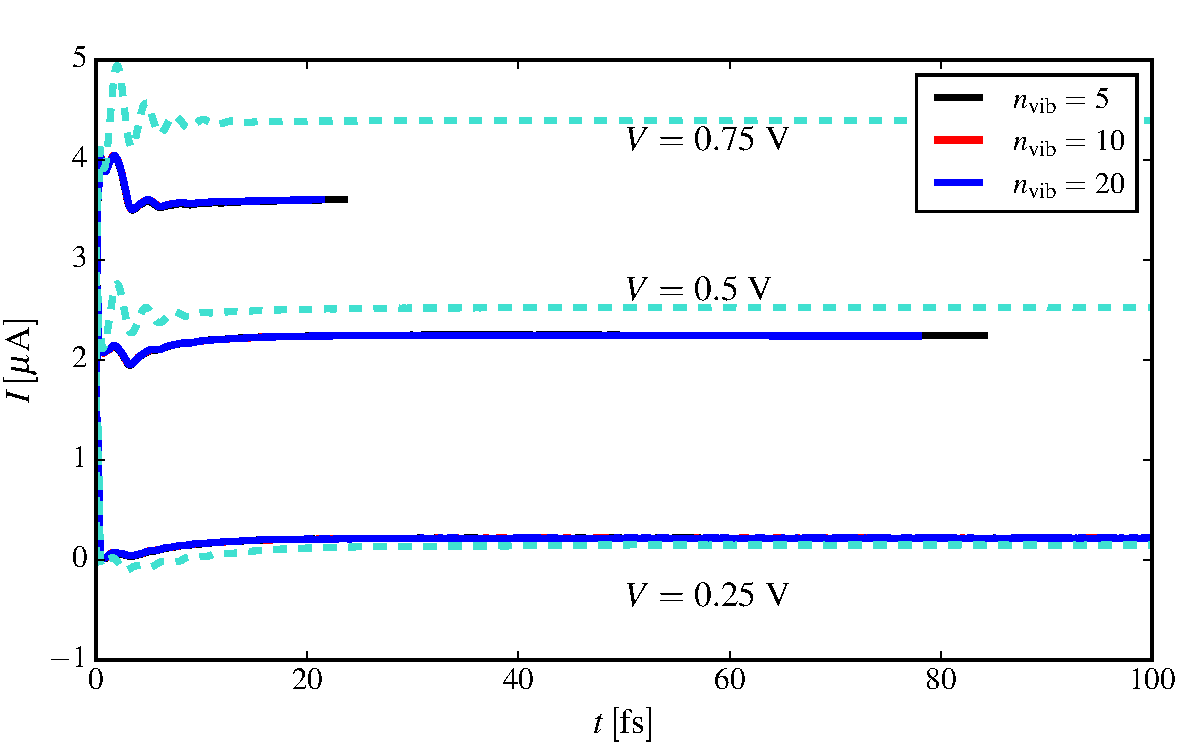
\includegraphics[width=0.54\textwidth]{figs/t1_8/L1x3_t1_8_tamen_cur_P_Vvar_nVar_tol1e-3.pdf}
	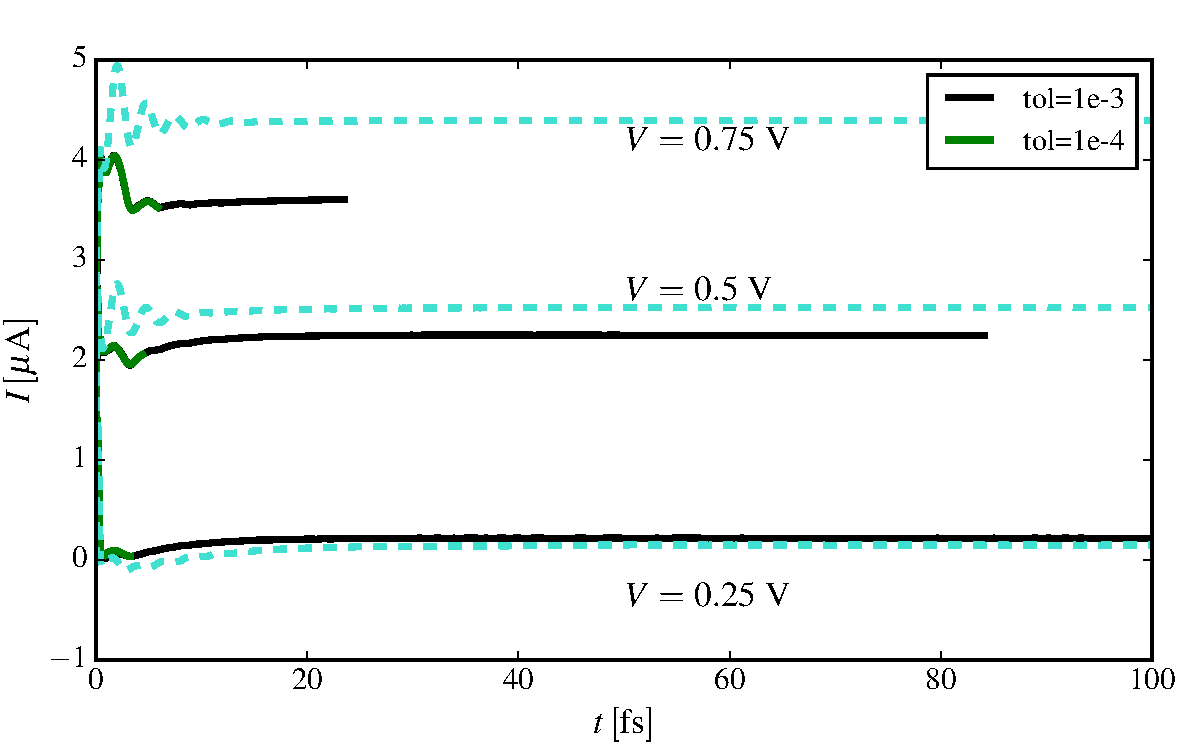
\includegraphics[width=0.54\textwidth]{figs/t1_8/L1x3_t1_8_tamen_cur_P_Vvar_nvib5_tolVar.pdf}
	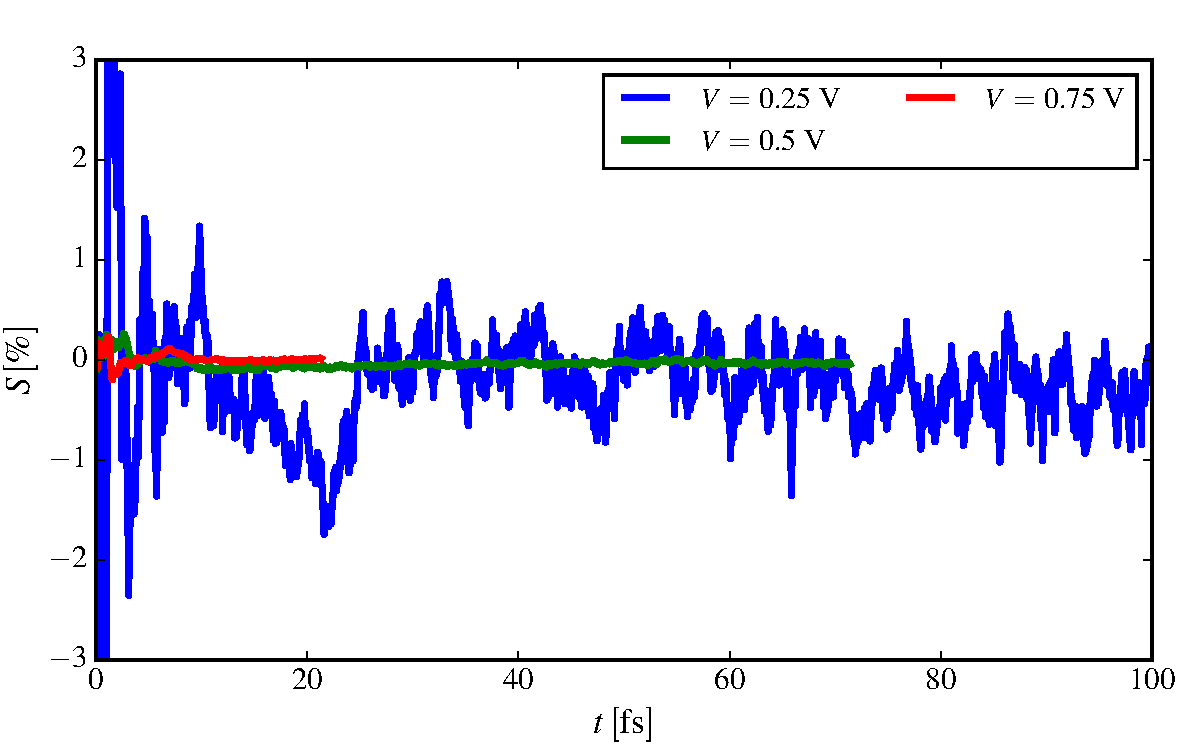
\includegraphics[width=0.54\textwidth]{figs/t1_8/L1x3_t1_8_tamen_SP_Vvar_nv20_tol1e-3.pdf}
	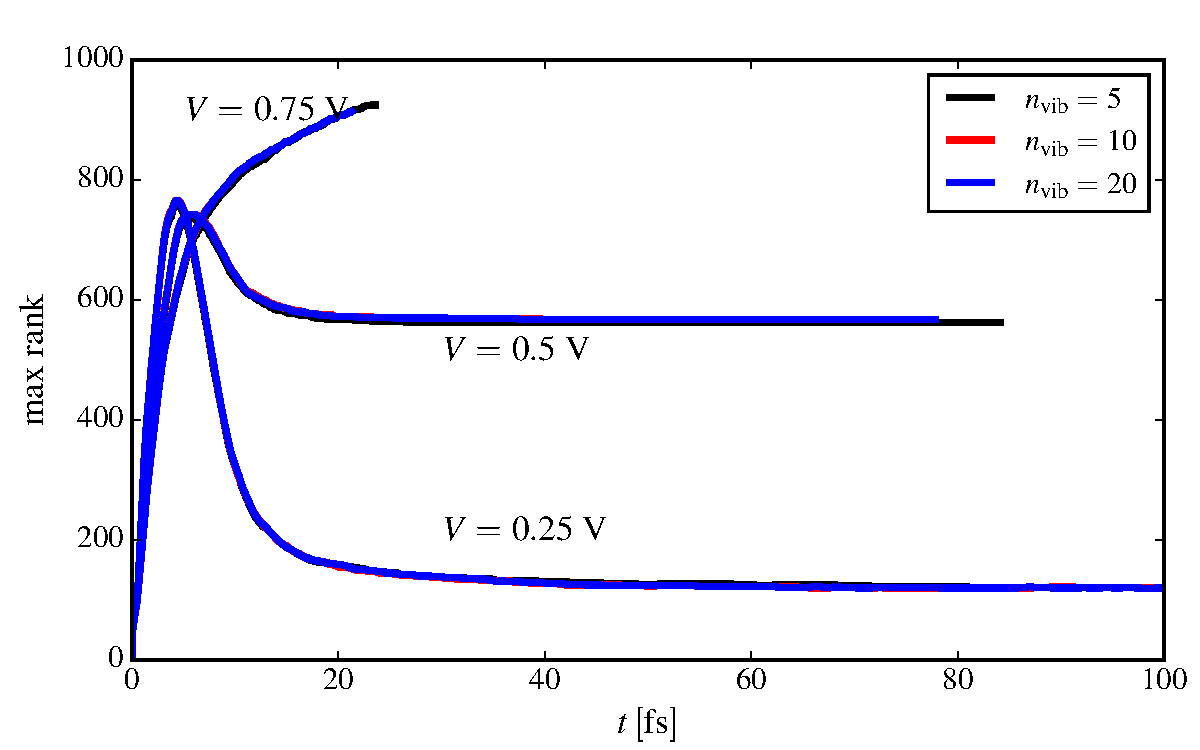
\includegraphics[width=0.54\textwidth]{figs/t1_8/L1x3_t1_8_tamen_maxRank_P_Vvar_nVar_tol1e-3.pdf}
\end{figure}


\end{document}


